%%%%%%%%%%%%%%%%%%%%%%%%%%%%%%%%%%%%%%%%%%%%%%%%%%%%%%%%%%%%%%%%%%%%%%%%%%%

\documentclass{standalone}

\usepackage{amsmath}
\usepackage{mathptmx}
\usepackage{pgfplots}
\usetikzlibrary{external}
\tikzexternalize{basel-problem-scatterplot}
\pgfplotsset{compat=1.15}

%% IEEE uses Times Roman font, so we'll default to Times.
%% These three commands make up the entire times.sty package.
\renewcommand{\rmdefault}{ptm}
\renewcommand{\ttdefault}{pcr}
\normalfont\selectfont

\begin{document}

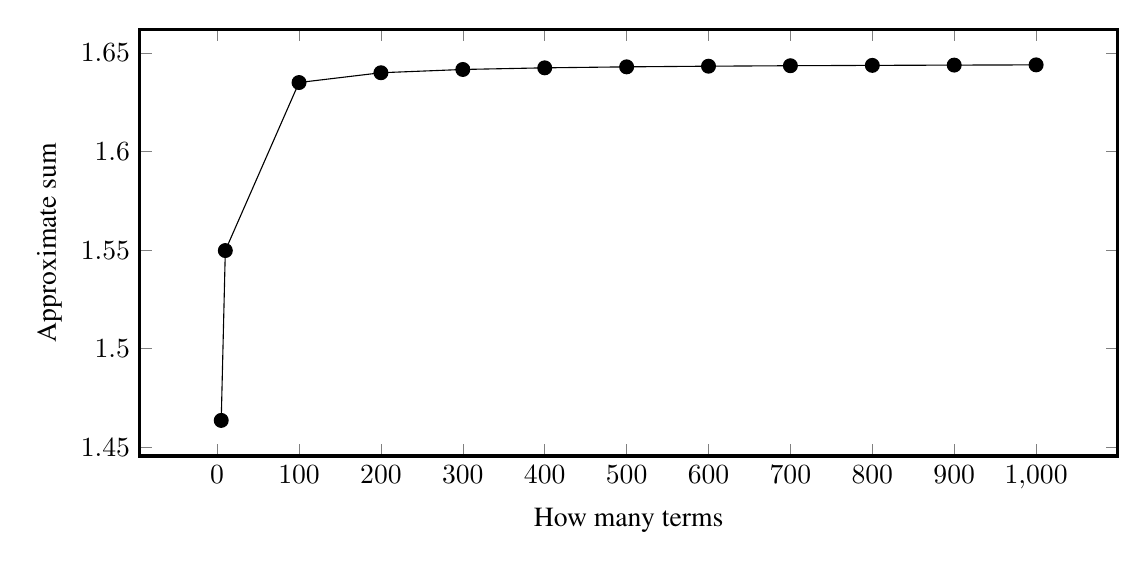
\begin{tikzpicture}
\tikzset{%%
  every mark/.append style={scale=1.0},%%
  scale=1.0%%
}
\pgfplotsset{%%
  every axis/.append style={font=\normalsize}%%
}
%%
\begin{axis}[%%
  axis line style=very thick,%%
  dotStyle/.style={mark size=2.5,black,mark color=black,mark=*},%%
  enlargelimits=true,%%
  height=7cm,%%
  plotStyle/.style={%%
    domain=4:17,%%
    mark=none,%%
    smooth,%%
    thick%%
  },%%
  width=14cm,%%
  xlabel={\normalsize How many terms},%%
  ylabel={\normalsize Approximate sum}%%
]
%%
%%
\addplot[dotStyle] coordinates {
  (5, 1.46361111111111)
  (10, 1.54976773116654)
  (100, 1.63498390018489)
  (200, 1.639946546015)
  (300, 1.64160628289762)
  (400, 1.64243718924406)
  (500, 1.64293606551489)
  (600, 1.64326878829884)
  (700, 1.64350651534191)
  (800, 1.6436848477727)
  (900, 1.64382357279244)
  (1000, 1.64393456668156)
};
\end{axis}
\end{tikzpicture}

\end{document}
